%%
% Please see https://bitbucket.org/rivanvx/beamer/wiki/Home for obtaining beamer.
%%
\documentclass{beamer}

\usepackage{amssymb,amsmath}

%\usepackage{refcheck}

\usepackage{graphicx}
\usepackage{amssymb}
\usepackage{mathrsfs}
\usepackage{amsmath}
\usepackage{latexsym}
\usepackage{amssymb}
\usepackage{enumerate}
\usepackage{color}
%\usepackage{ dsfont }
\usepackage{float}
\usepackage{physics}

%new math symbols taking no arguments
\newcommand\0{\mathbf{0}}
\newcommand\CC{\mathbb{C}}
\newcommand\FF{\mathbb{F}}
\newcommand\NN{\mathbb{N}}
\newcommand\QQ{\mathbb{Q}}
\newcommand\RR{\mathbb{R}}
\newcommand\ZZ{\mathbb{Z}}
\newcommand\bb{\mathbf{b}}
\newcommand\kk{\Bbbk}
\newcommand\mm{\mathfrak{m}}
\newcommand\pp{\mathfrak{p}}
\newcommand\xx{\mathbf{x}}
\newcommand\yy{\mathbf{y}}
\newcommand\GL{\mathit{GL}}
\newcommand\into{\hookrightarrow}
\newcommand\nsub{\trianglelefteq}
\newcommand\onto{\twoheadrightarrow}
\newcommand\minus{\smallsetminus}
\newcommand\goesto{\rightsquigarrow}
\newcommand\nsubneq{\vartriangleleft}

%redefined math symbols taking no arguments
\newcommand\<{\langle}
\renewcommand\>{\rangle}
\renewcommand\iff{\Leftrightarrow}
\renewcommand\phi{\varphi}
\renewcommand\implies{\Rightarrow}

%new math symbols taking arguments
\newcommand\ol[1]{{\overline{#1}}}

%redefined math symbols taking arguments
\renewcommand\mod[1]{\ (\mathrm{mod}\ #1)}

%roman font math operators
\DeclareMathOperator\aut{Aut}

%for easy 2 x 2 matrices
\newcommand\twobytwo[1]{\left[\begin{array}{@{}cc@{}}#1\end{array}\right]}

%for easy column vectors of size 2
\newcommand\tworow[1]{\left[\begin{array}{@{}c@{}}#1\end{array}\right]}


\title{Quantum-inspired $\ell^2$ sampling}
\subtitle{and applications to machine learning}
\author[Sbahi] % (optional, for multiple authors)
{Faris Sbahi}
\date{3/5/19}
\subject{Physics}

\begin{document}
\maketitle

\AtBeginSection[]
{
  \begin{frame}<beamer>
    \tableofcontents[currentsection]
  \end{frame}
}

\section{Machine Learning}

\begin{frame}
    \frametitle{Machine Learning}
    \framesubtitle{Introduction}
    \begin{itemize}
    \item Machine learning is a broad term for algorithms which are capable of finding patterns in data.
    \item Fundamental goal: capture these patterns in a "model" that \textit{generalizes}.
    \item These algorithms have two components:
    \begin{enumerate}
    \item A learning element. Updates the model depending on its performance on the considered dataset.
    \item A performance element. Provides the measure of performance.
    \end{enumerate}
	\item Bottom line: "machine learning" is a somewhat hollow term. Many ML algorithms are in fact familiar linear algebraic techniques.
    \end{itemize}
    \end{frame}

% Goal is simply to show why these linear algebraic techniques can be regarded as machine learning algorithms
  \begin{frame}
  	\frametitle{PCA}
    \framesubtitle{Motivation: Singular value transformation}
    \begin{itemize}
    \item "Training" dataset $\mathcal{T}$ consists of the accessible samples of data. $\mathcal{T}$ is drawn from a subset of $\Omega \subset \RR^d$ where each component represents a "feature". 
    \item Samples from $\Omega$ are assumed to be drawn according to some distribution $\mathcal{D}$. 
    \item Example: data is collected on the heights and lengths of cherry blossom petals. 
    \begin{figure}
   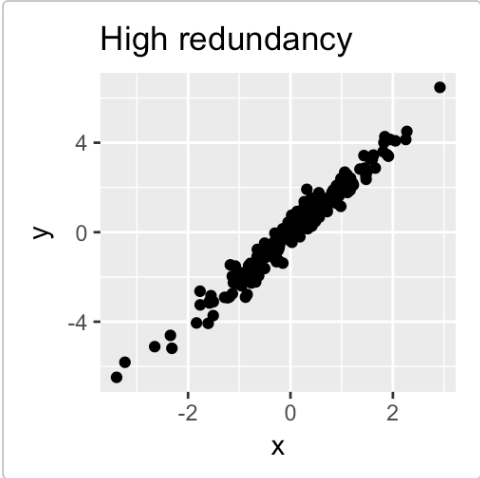
\includegraphics[width= 0.3\linewidth]{pca_high_redundancy.png}
   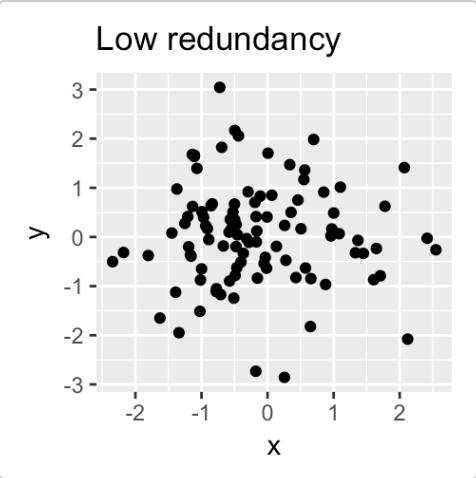
\includegraphics[width= 0.3\linewidth]{pca_low_redundancy}	
\end{figure}
\item How and why may it make sense to reduce the dimensionality of the feature space?
\end{itemize}
\end{frame}

\begin{frame}
\frametitle{Moore-Penrose Pseudoinverse}
    \framesubtitle{Motivation: Singular value transformation}
    \begin{itemize}
    \item Say we wish to solve the linear system 	
    \end{itemize}
	
\end{frame}


\section{Quantum Machine Learning}

\begin{frame}
\frametitle{}	
\end{frame}


\section{Classical $\ell^2$ sampling}

% polynomial transformations on singular values
  
% Our work gives evidence that this conversion can be done in general for low-rank problems, suggesting that exponential quantum speed-ups are tightly related to problems where high-rank matrices play a crucial role, like in Hamiltonian simulation or the Fourier transform.

 \end{document}
  
